\documentclass{article}
\usepackage[utf8]{inputenc}
\usepackage{graphicx}
\usepackage{float}

\title{Comprehensive Analysis of the Chile Real Estate Market}
\author{Olubayode Ebenezer}
\date{\today}

\begin{document}

\maketitle

\section*{Abstract}
This document provides a comprehensive analysis of the Chile real estate market, delving into the variety of property types, prices, sizes, and geographical locations present within the dataset. The data forms the basis for a detailed examination of the market dynamics, price trends, and geographical distribution of properties, aiming to present a clear view of the real estate landscape in Chile.

\section{Introduction}
The Chilean real estate market is dynamic and diverse. A rigorous analysis requires a dataset that is both comprehensive and meticulously cleaned to ensure reliable results. This report encapsulates every phase of the data cleaning process, highlighting the importance of each step to ensure the data's integrity.

\section{Data Cleaning Process}
\subsection{Removing Duplicates}
The initial phase involved removing duplicate entries based on the 'id' column to guarantee the uniqueness of each listing.

\subsection{Quality Report Function}
A tailored function, \texttt{quality\_report}, was developed to evaluate the dataset systematically. It provided insights into the missing values, unique values count, and data types across columns, which was instrumental for guiding the cleaning process.

\subsection{Dropping Unnecessary Columns}
To refine the dataset, columns such as 'expenses', 'price\_per\_m2', 'place\_with\_parent\_names', and 'price\_usd\_per\_m2' were eliminated due to their redundancy or lack of relevance for the analysis.

\subsection{Handling Missing Values}
This critical stage aimed to enhance the quality of the dataset. Rows and columns with missing data were scrutinized, with removal or imputation decisions based on their analytical importance and the degree of missing information. A boxplot visualization was employed to identify and subsequently remove outliers in the 'expenses' column.

For the 'currency' column, missing values were substituted with a default value of 0. Key numerical columns, including 'price', 'price\_aprox\_usd', and 'surface\_total\_in\_m2', had their missing values replaced with the mean to prevent the introduction of bias and preserve the integrity of the analysis.

\subsection{Distribution Analysis of Numerical Features}
The \texttt{numeric\_distribution\_plot} function was created to visualize the distribution of numerical features, helping to pinpoint outliers and comprehend the data spread.

\subsection{Visualizing Data Cleanliness}
Post-cleanup, a heatmap was employed to visually affirm the cleanliness of the data, indicating the absence of significant missing information. Additionally, distribution plots for 'price' and 'rooms' corroborated the normality of the data distribution after the cleaning steps.

\subsection{Final Adjustments}
The dataset's simplification was furthered by removing the 'price\_aprox\_local\_currency' column, with an inferred preference for analyzing prices in USD for streamlined analysis.

The meticulous cleaning process rendered the dataset not just neat but also suitable for in-depth analytical endeavors. This transformation underscores the cleaned dataset's reliability for further analyses, ensuring the data is representative and trustworthy.

\section{Visualization Insights and Interpretations}
\subsection{Linear Model Plot: Price vs. Rooms}
\begin{figure}[H]
\centering
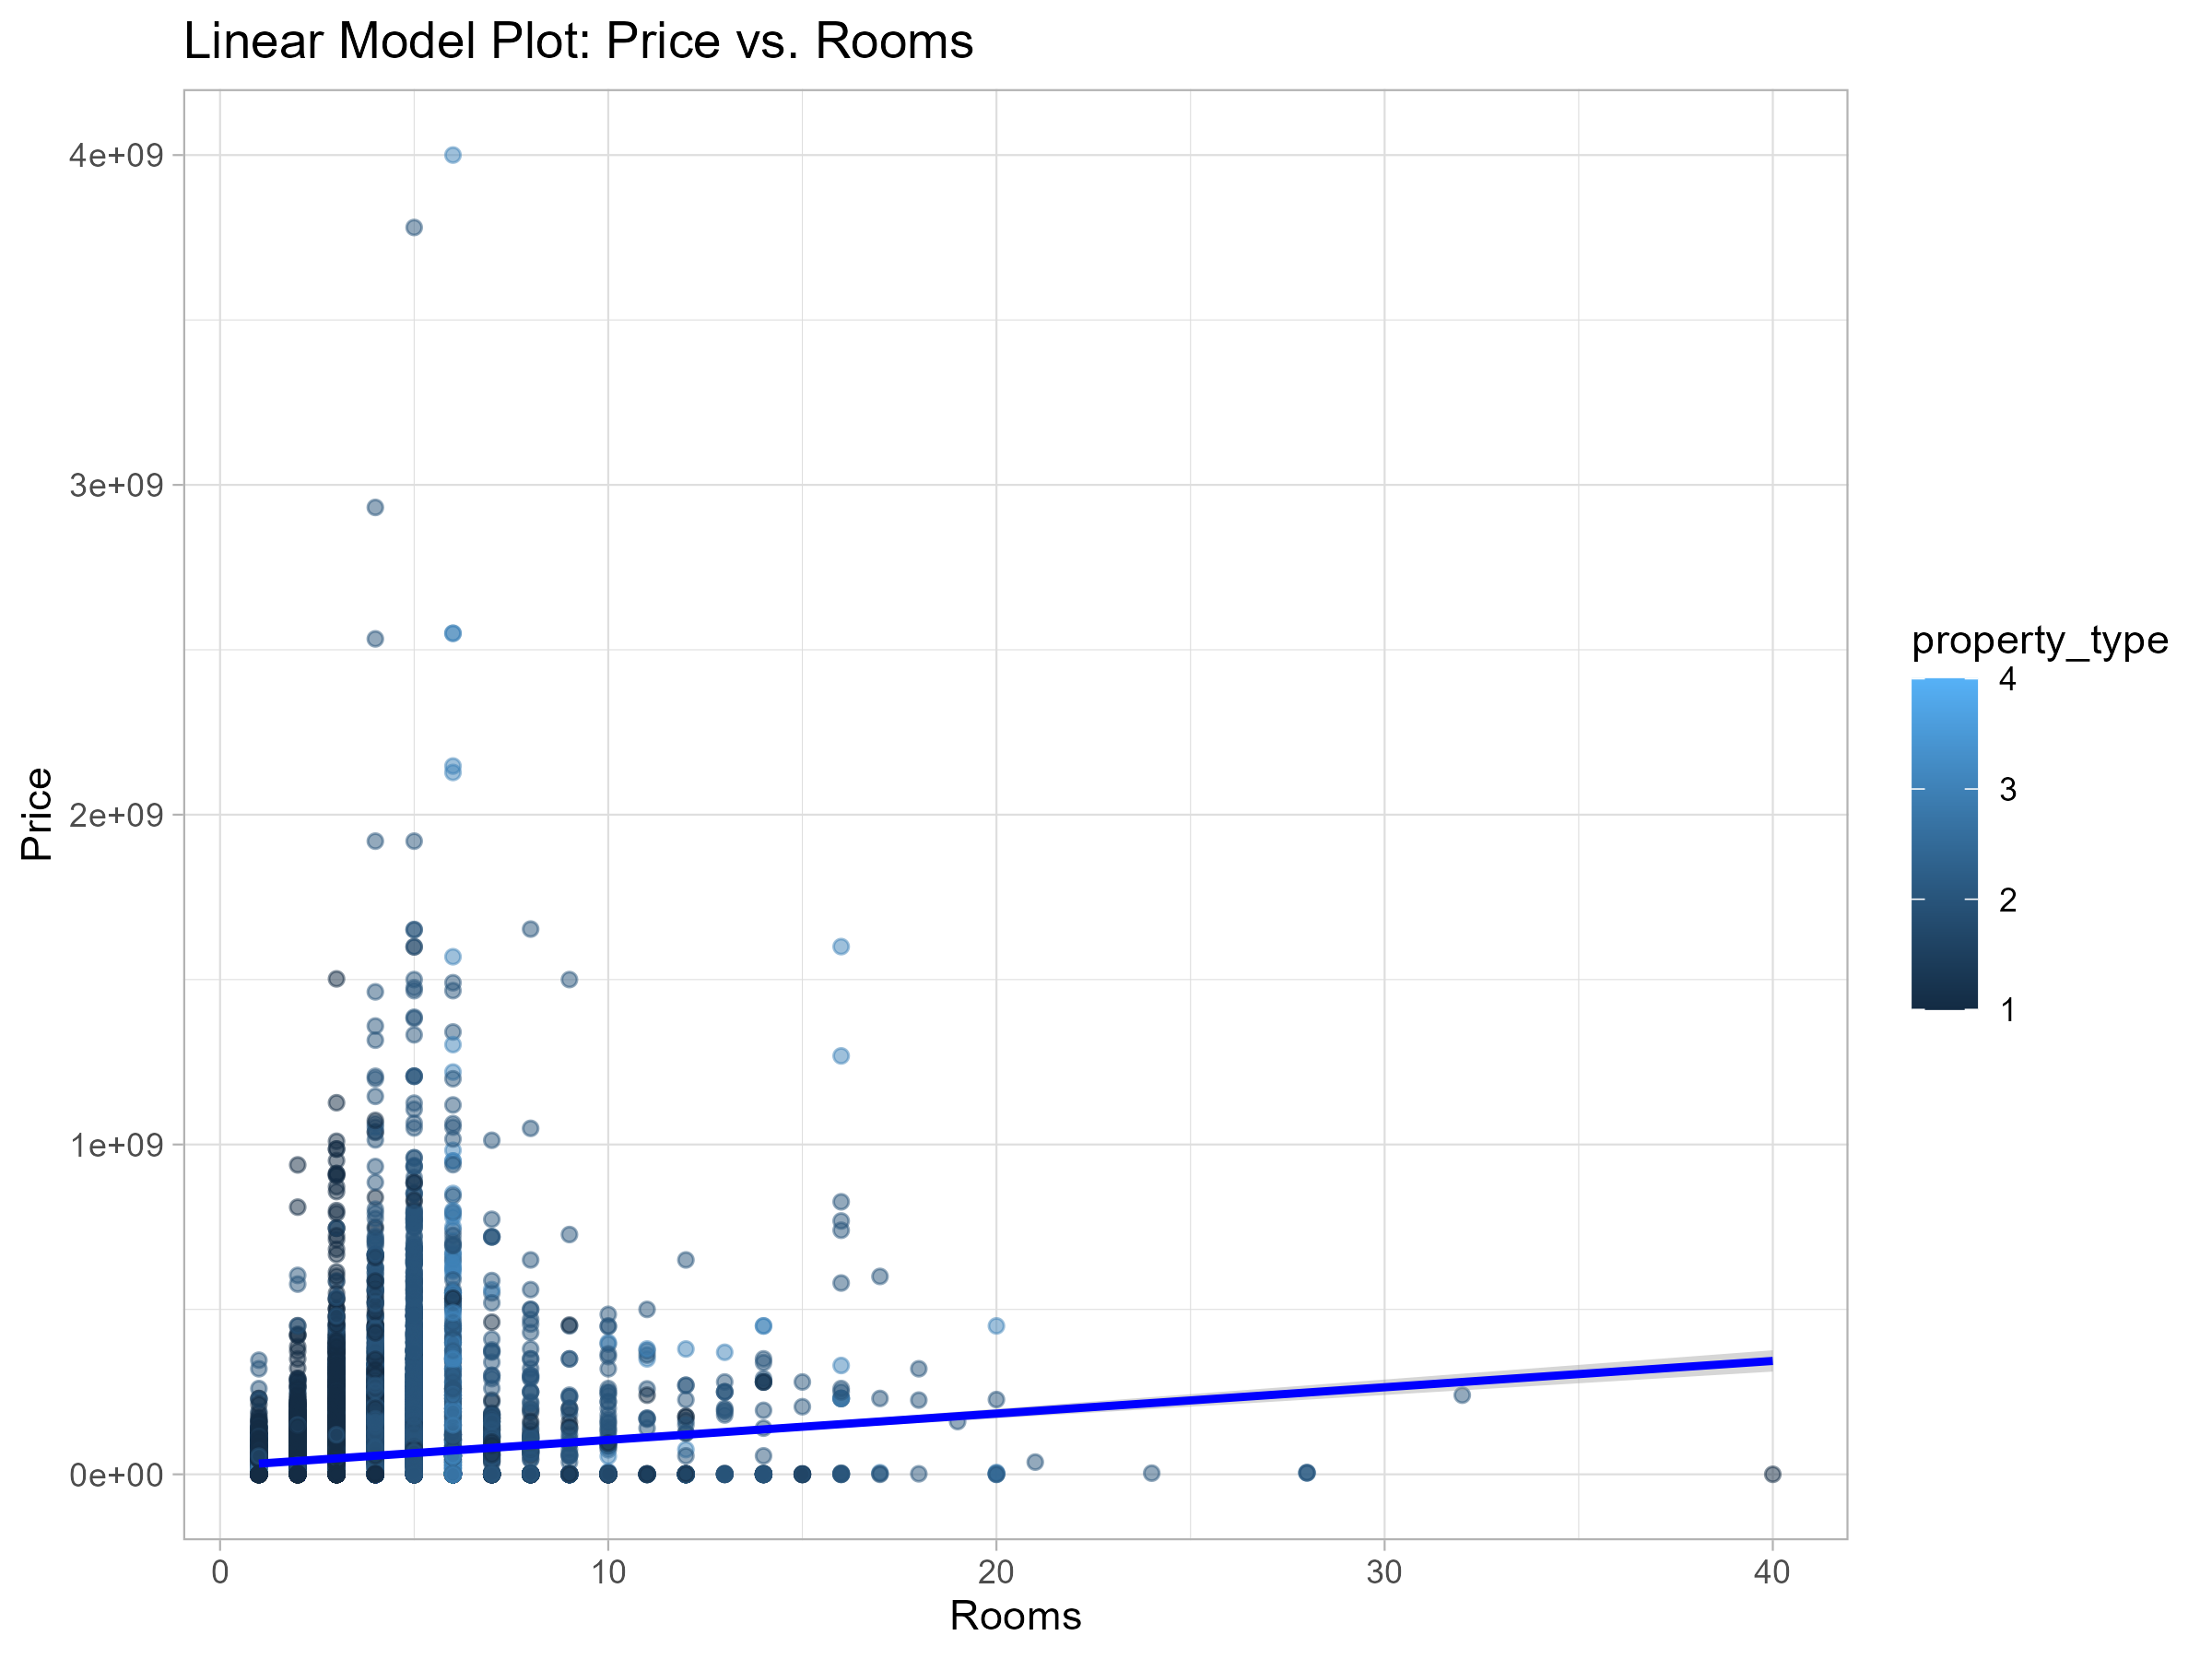
\includegraphics[width=\textwidth]{PS6b_Olubayode.png}
\caption{Linear model plot showing the relationship between the number of rooms and property prices.}
\end{figure}

The lmplot visualized a seemingly paradoxical trend: properties with more rooms tend to have lower prices. This negative correlation suggests that, on average, a higher room count may not command higher property prices.

\subsection{Economic and Market Dynamics Interpretation}
The insight derived from the plot is that the value per room diminishes as the total number of rooms increases. This can be attributed to factors such as economies of scale, market demand, and the functional utility of the properties. For instance, In Economies of Scale: Larger properties, with their increased number of rooms, might not proportionally increase in price due to economies of scale. This could make individual rooms in such properties more cost-effective, appealing to buyers seeking more space for their investment.

\subsection{Conclusion from Linear Model Plot}
This analysis challenges the notion that a higher room count unequivocally results in higher property prices. It exposes the intricate balance between property size, utility, demand, and pricing, critical for stakeholders in the real estate industry.

\section{Room Distribution Insights}
\subsection{Bar Plot: Average Rooms by Property Type}
\begin{figure}[H]
\centering
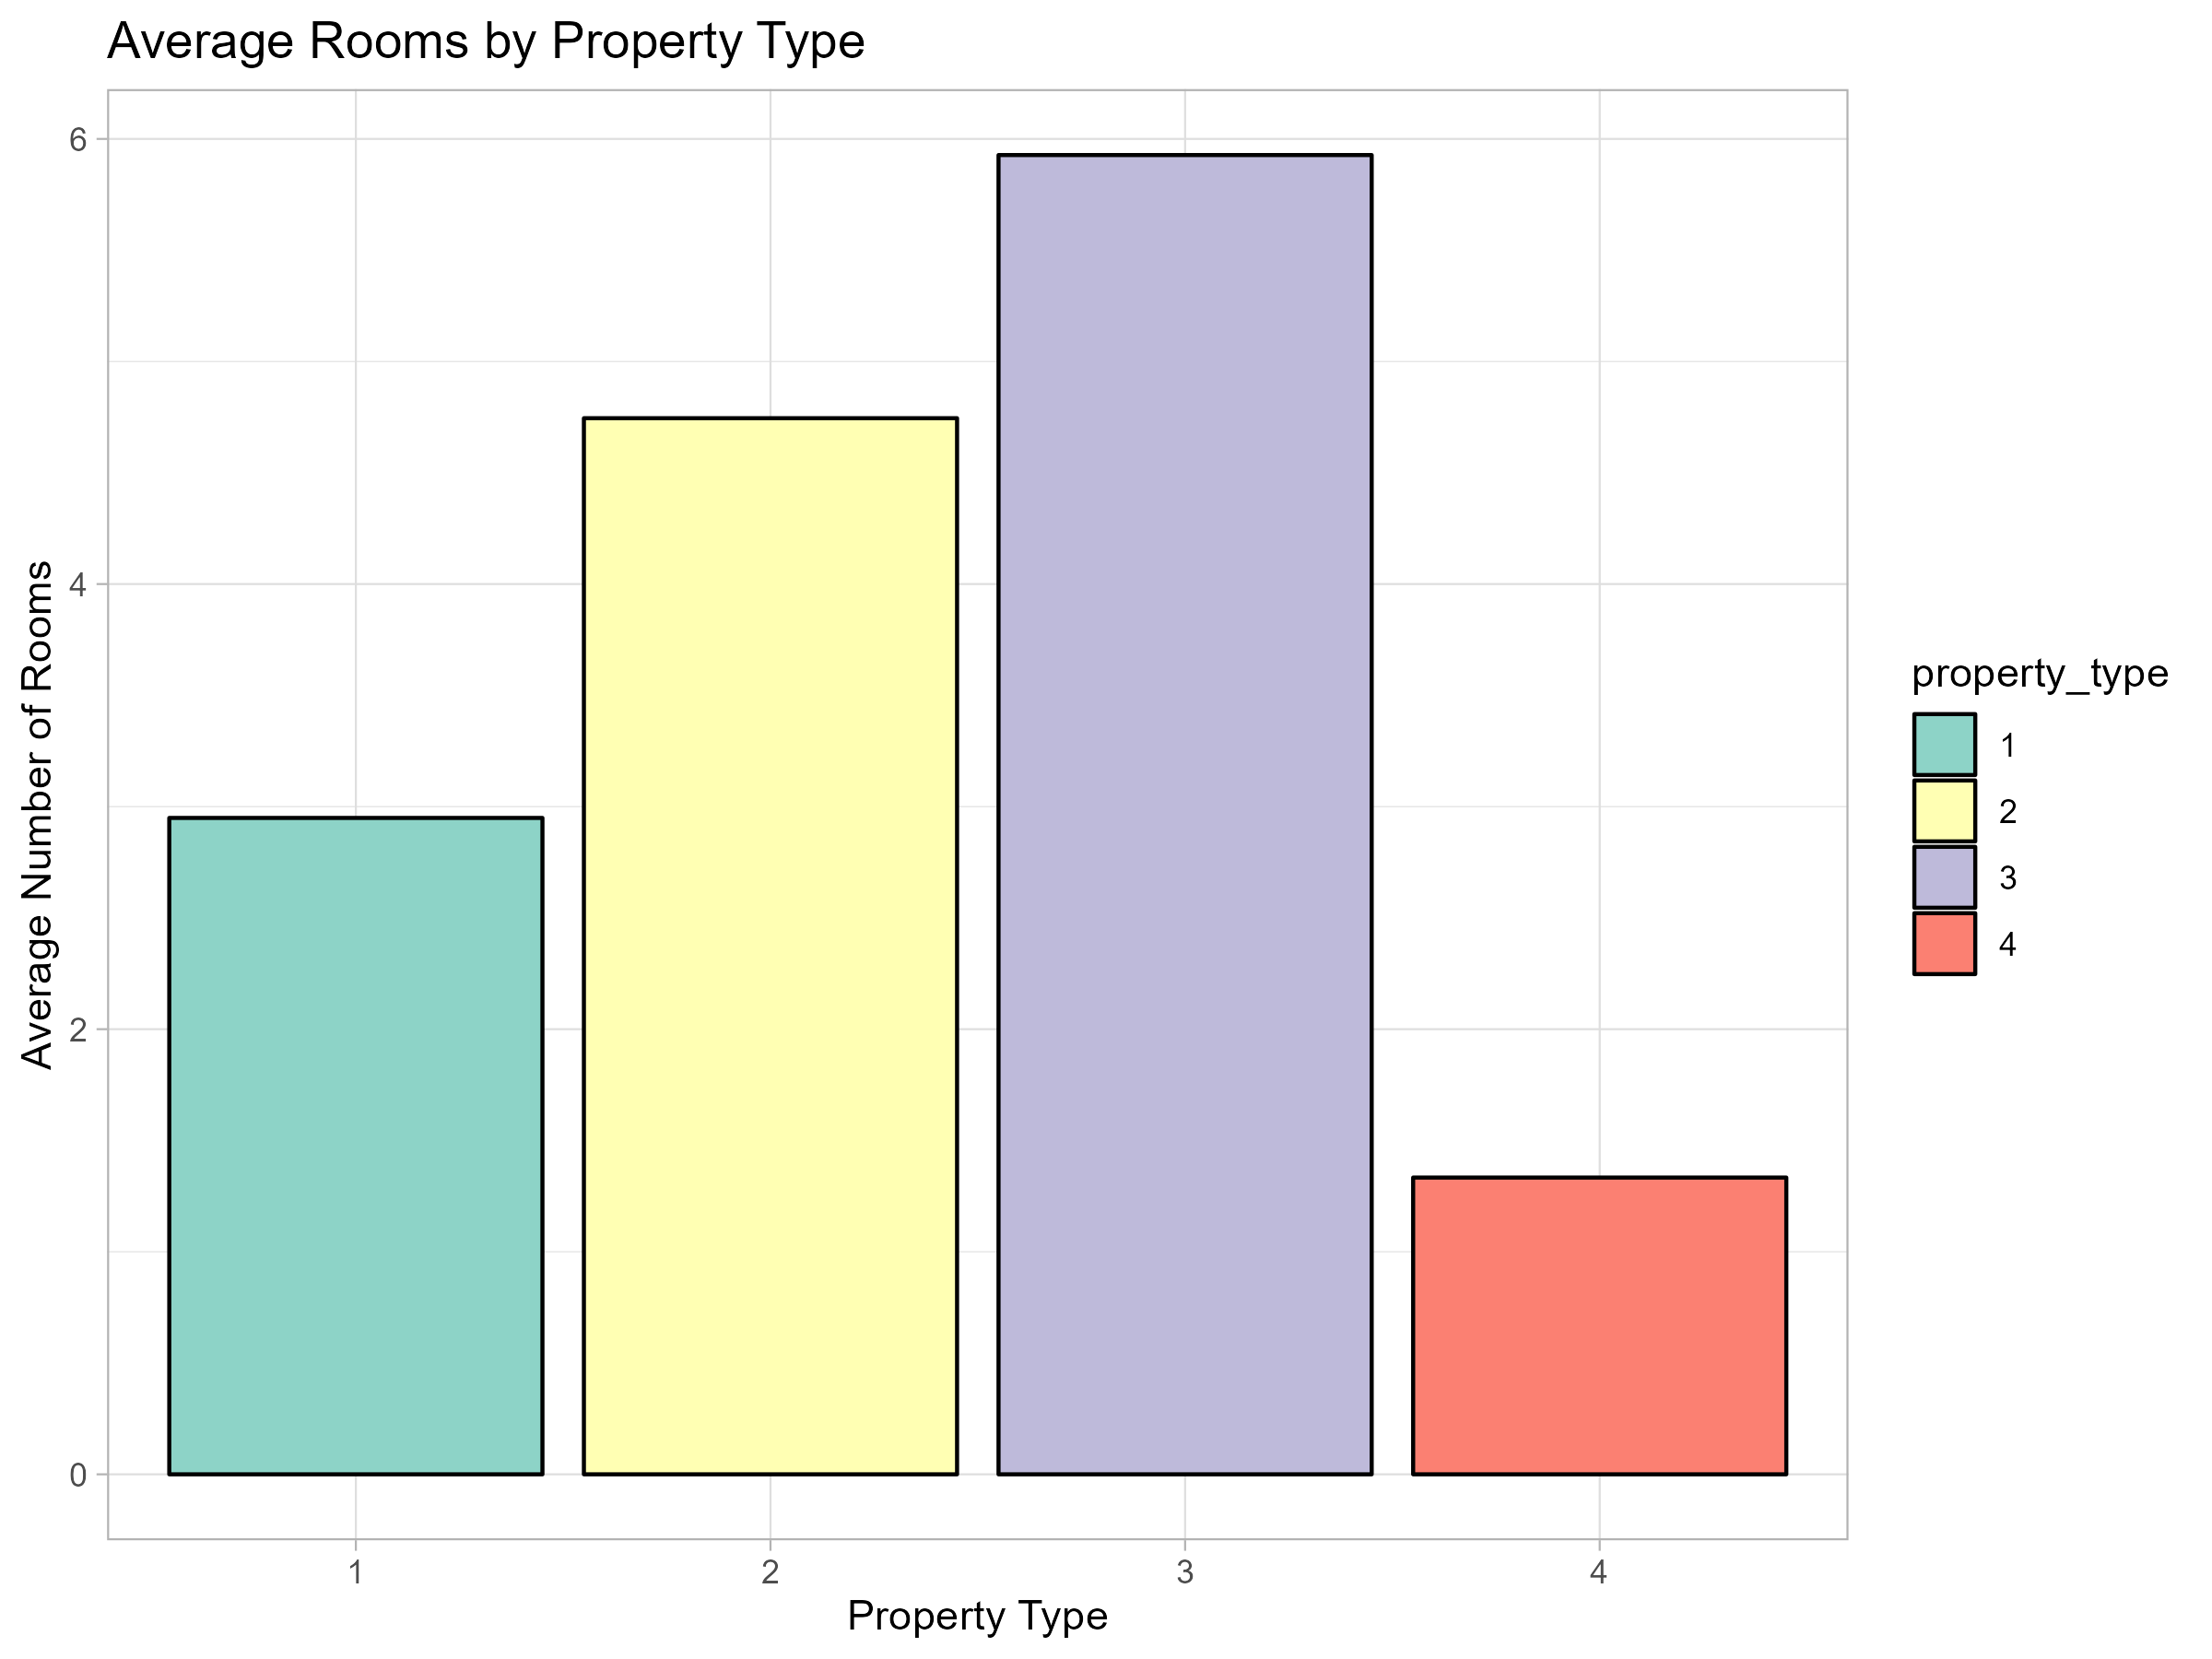
\includegraphics[width=\textwidth]{PS6c_Olubayode.png}
\caption{Average number of rooms across different property types.}
\end{figure}

The bar plot offers insights into the average room count across different property types categorized numerically. The analysis reveals the following:
\begin{itemize}
\item \textbf{Property Type 1 (Apartments):} The average number of rooms for apartments indicates a moderate count, which aligns with the typical expectations for such properties where living space efficiency is often balanced with locational advantages.
\item \textbf{Property Type 2 (Houses):} Houses show the highest average room count, reflecting their general design for more spacious living and their suitability for families or larger living arrangements.
\item \textbf{Property Type 3 (Stores):} Stores present a room count that is less than that of houses but more than apartments, possibly indicating the inclusion of additional storage or operational spaces beyond the main commercial area.
\item \textbf{Property Type 4 (PH):} 'PH' properties have the lowest average room count among the categories, suggesting they are smaller units, possibly akin to condominiums or flats with limited living space.
\end{itemize}

\subsection{Pie Chart: Room Distribution in Property Types}
\begin{figure}[H]
\centering
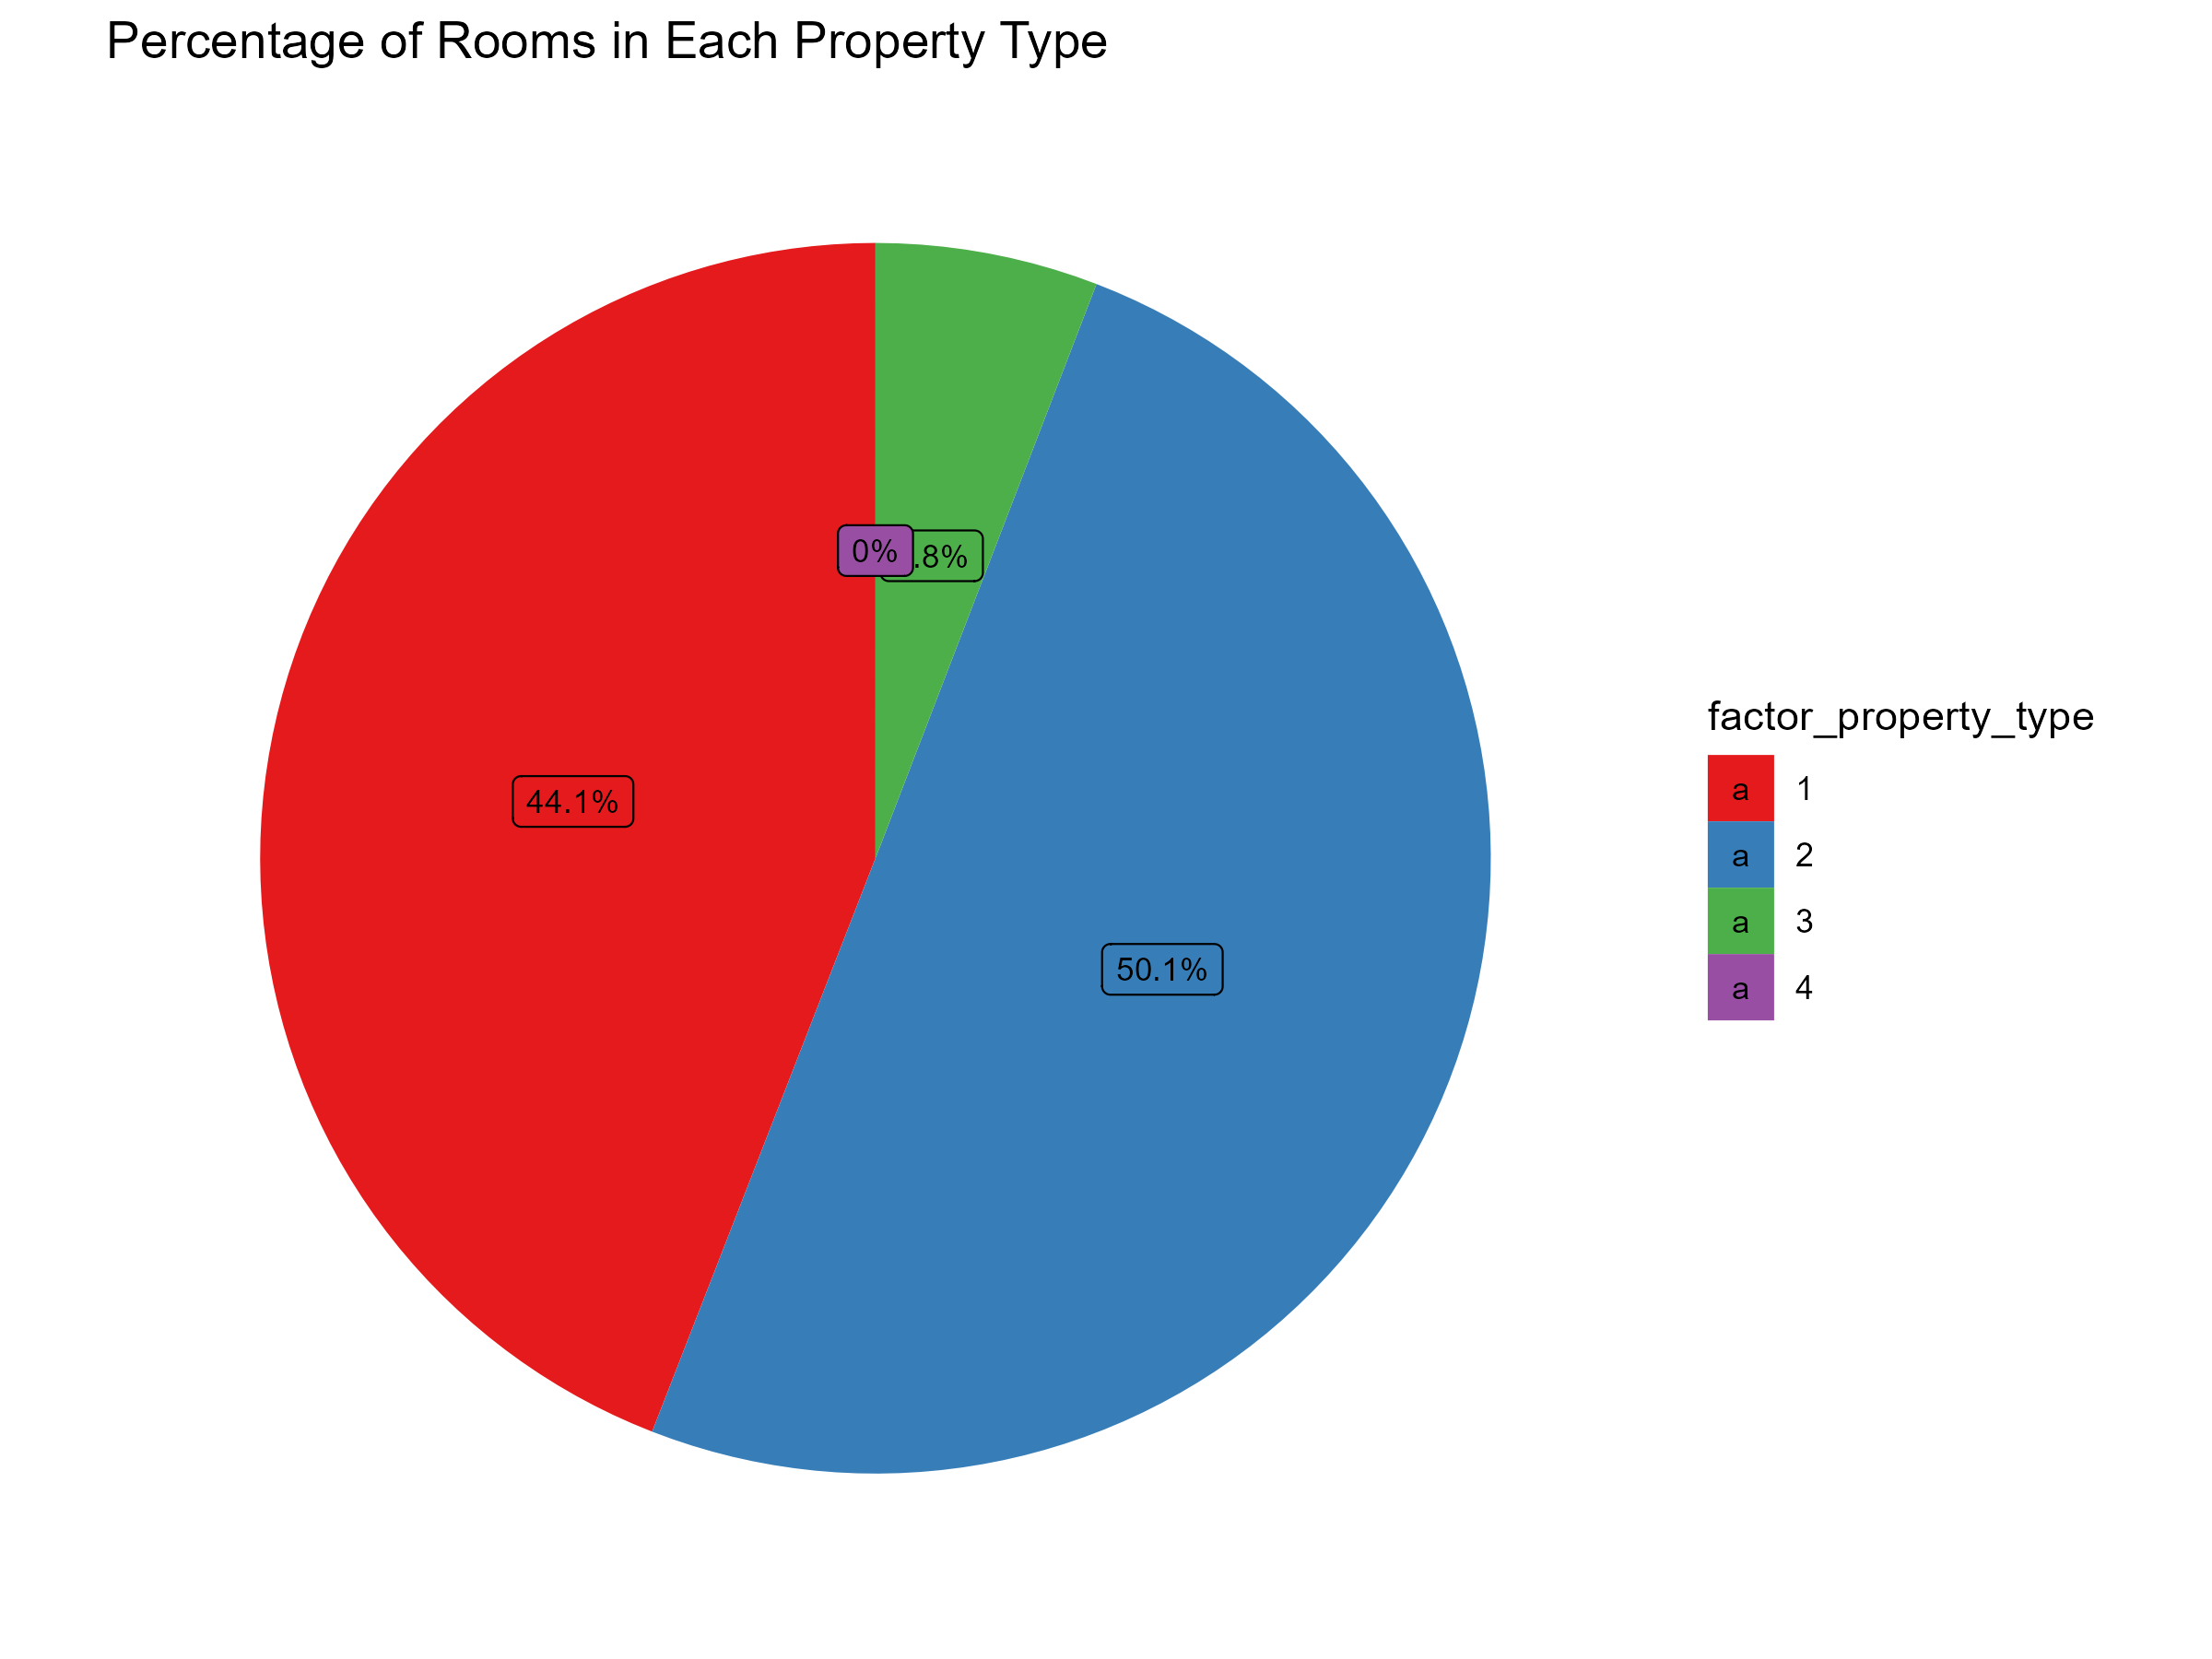
\includegraphics[width=\textwidth]{PS6d_Olubayode.png}
\caption{Proportional distribution of rooms in different property types.}
\end{figure}

The pie chart visualizes the proportion of total rooms attributed to each property type:
\begin{itemize}
\item \textbf{Property Type 1 (Apartments):} Apartments constitute 44.1\% of the total room count, underscoring their significant presence in the real estate market.
\item \textbf{Property Type 2 (Houses):} With 50.1\%, houses account for the majority of rooms, likely due to their design for more roomy living spaces.
\item \textbf{Property Type 3 (Stores):} Stores account for 5.8\%, which, while lower in comparison to houses and apartments, is still substantial, suggesting a prevalence of mixed-use or workspace-oriented properties.
\item \textbf{Property Type 4 (PH):} PH properties represent a minimal fraction, potentially indicative of a smaller market presence or a preference for fewer rooms within these property types.
\end{itemize}

\subsection{Relationship to the Data:}
The data reflected in both visualizations capture the typical configurations of the Chilean real estate market, with a balanced mix of apartments and houses catering to different market segments. The insights derived from these figures are invaluable for stakeholders such as investors, developers, and policymakers, as they provide a clear understanding of how living spaces are distributed across property types in the market.


i.e The bar plot and pie chart collectively offer a granular view of the room distribution across various property types in the dataset. They illustrate the expected trends and provide market composition insights, serving as valuable resources for investors and policymakers alike.



\section{Heatmaps: Before and After Data Cleaning}
\subsection{Prior to Data Cleaning}
\begin{figure}[H]
\centering
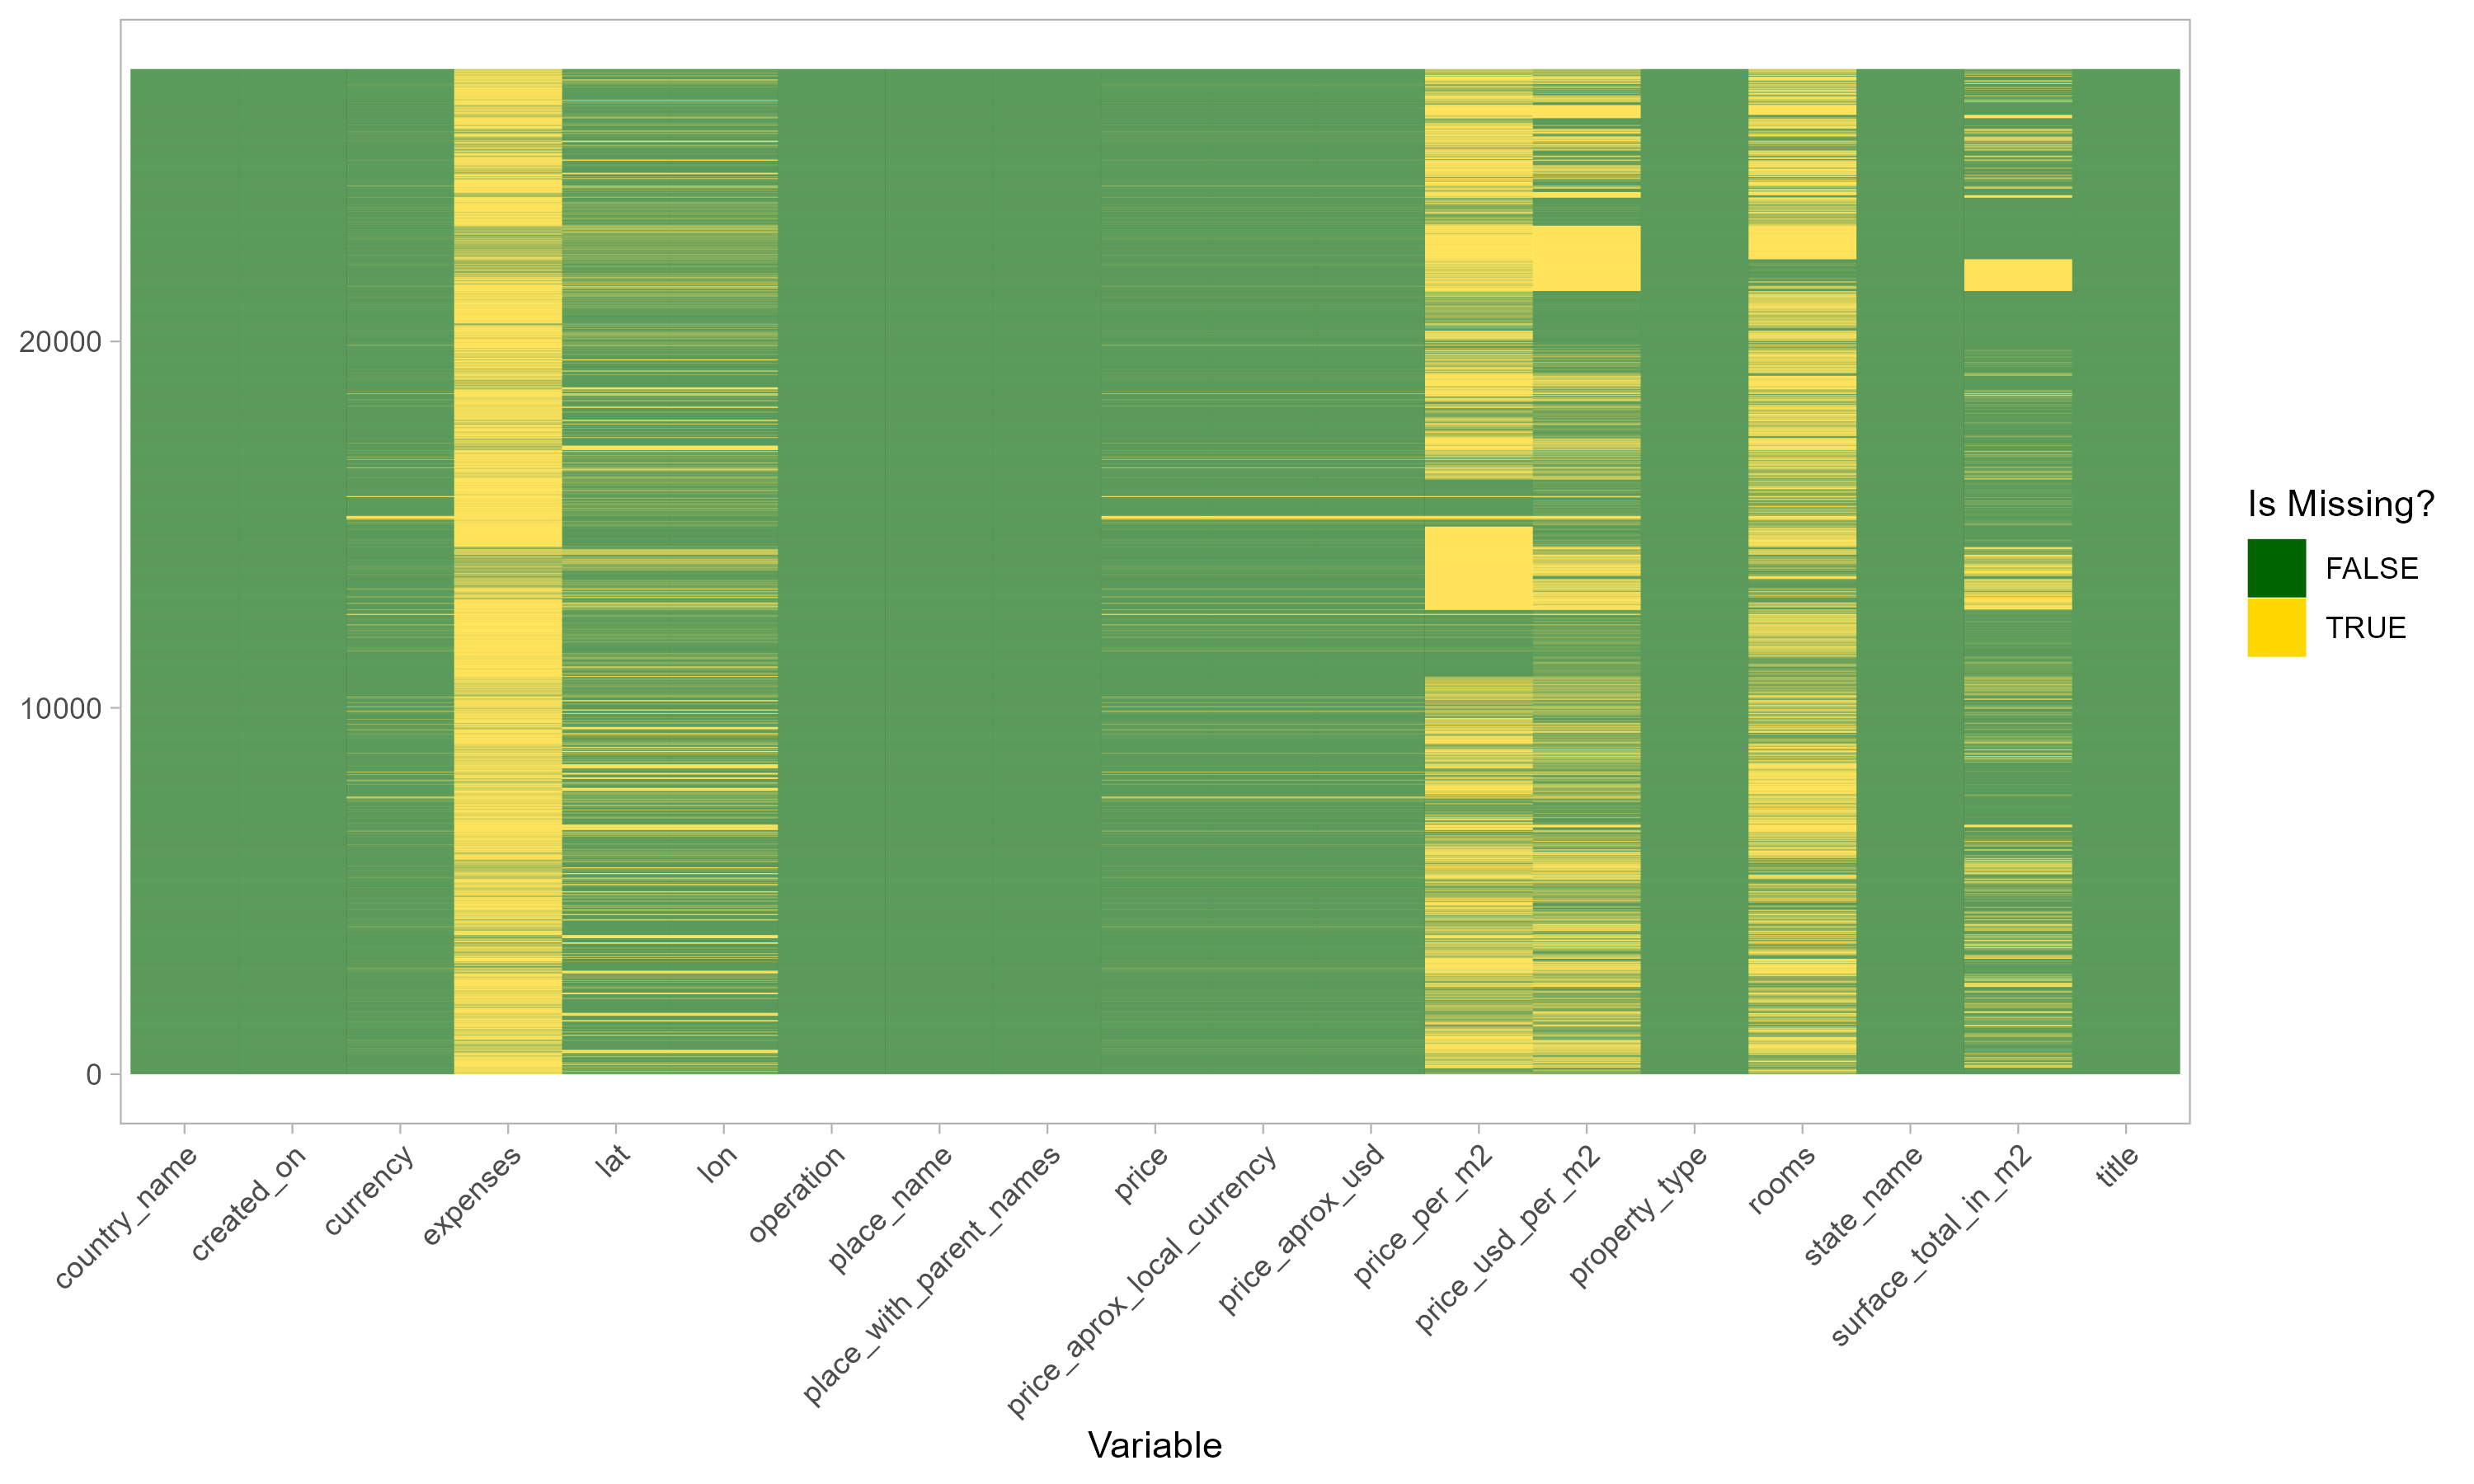
\includegraphics[width=\textwidth]{PS6a_Olubayode.png}
\caption{Heatmap indicating the presence of missing data before the cleaning process.}
\end{figure}

The heatmap showcases the extensive missing data across several variables, signaling the necessity for thorough cleaning.

\subsection{After Data Cleaning}
\begin{figure}[H]
\centering
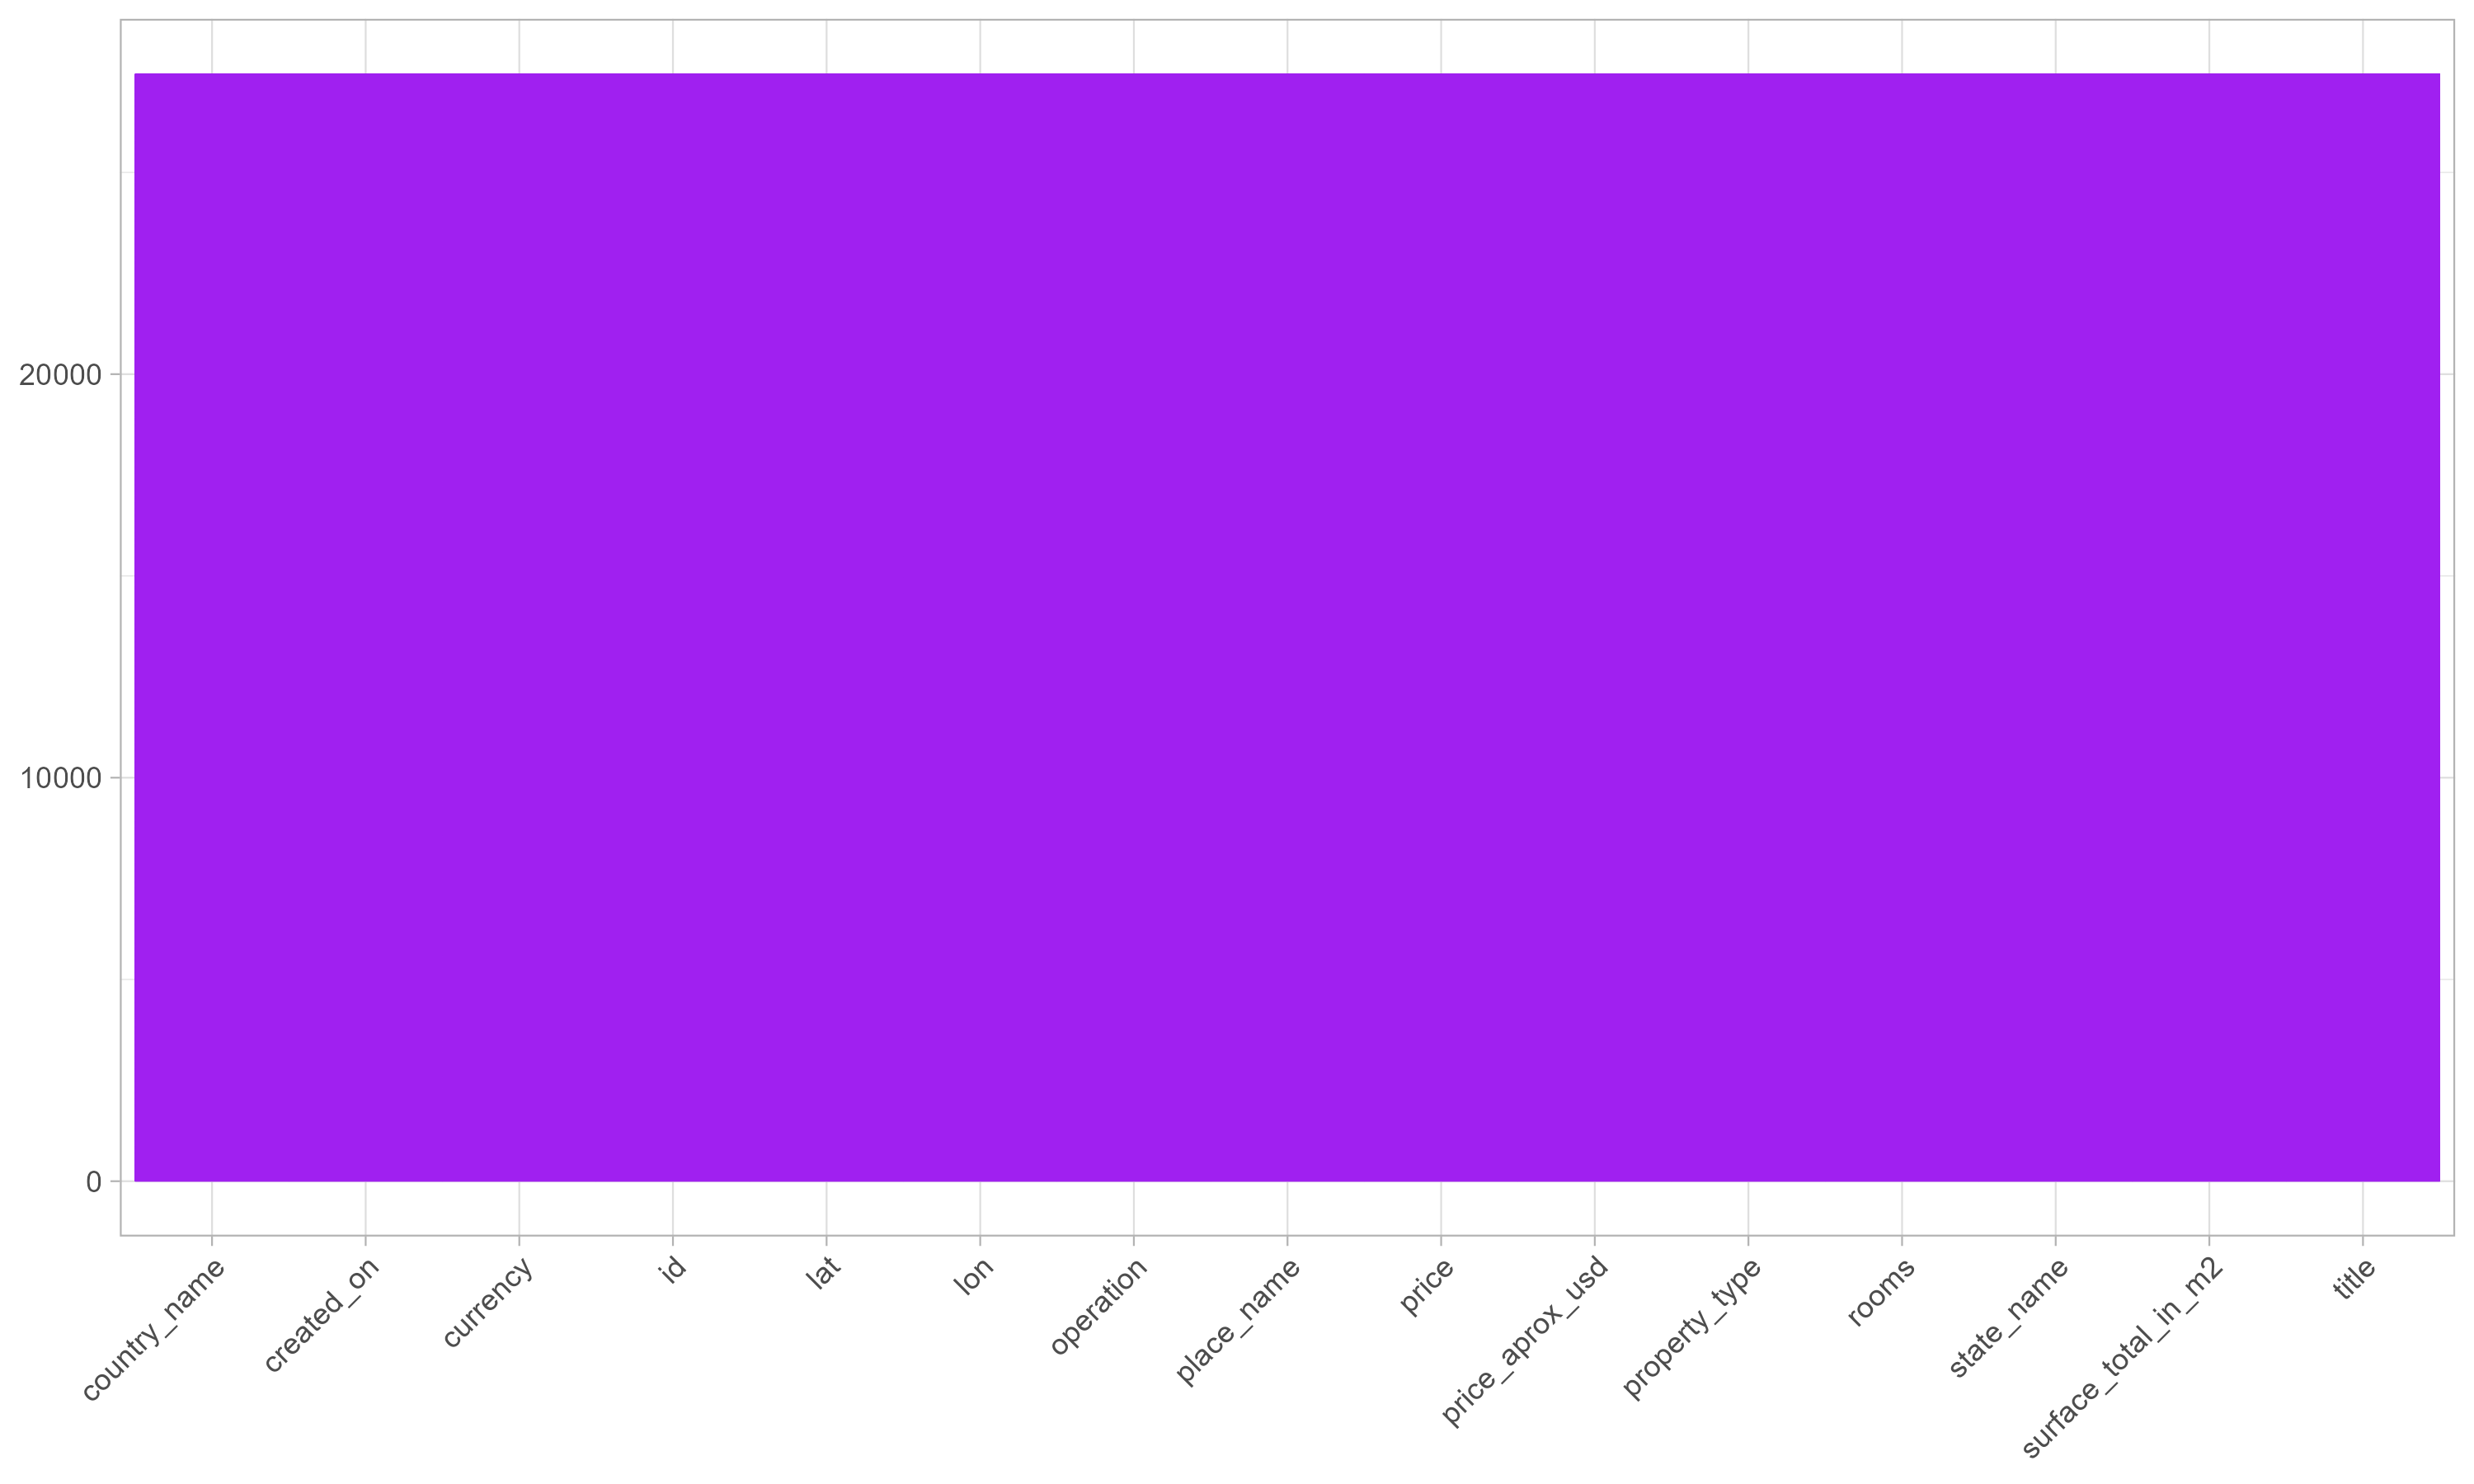
\includegraphics[width=\textwidth]{PS6e_Olubayode.png}
\caption{Heatmap showing the absence of missing data following the cleaning process.}
\end{figure}

Post-cleaning, the heatmap demonstrates a dataset free from missing values, affirming the effectiveness of the cleaning process and setting a strong foundation for accurate analysis.

\section{Conclusion}
The cleaning process and the subsequent analyses provided deep insights into the Chile real estate market. The heatmaps served not only as a tool for identifying and rectifying data quality issues but also as a testament to the thoroughness of the cleaning process. This rigorous approach ensures the dataset's integrity, which is indispensable for any substantial real estate market analysis.

\end{document}
